\documentclass{article}
\usepackage {inputenc, fullpage, listings, amsmath, graphicx}

\lstset{
         numbers=left,               
         stepnumber=1,                
         numberfirstline=false
 }

\parindent 0pt

\title{%
   ECE 458 (Spring 2022) Assignment 2 \\
   \large Alex Holland V00}
    
\date{}

\begin{document}

\maketitle

{\bf Question 1}\\
{\bf (a)}\\
The time (in msec) that elapses from when you click on the link until you receive the object can be represented by $RTT_0+RTT_1+2 \times RTT_{HTTP}$. Two $RTT_{HTTP}$ is required in order to establish the TCP connection and perform an HTTP GET response. Thus the total time is $2msecs+48msecs+2 \times (16msecs)=82msecs$

\bigskip
{\bf (b)}\\
For each of the 2 embedded objects, a delay of $RTT_{HTTP}$ is required to establish the TCP connection and also to perform an HTTP GET response. One $RTT_{HTTP}$ to establish a a TCP connection, and another to send and receive the HTTP request. Thus the time (in msec) that elapses from when you click on the link until the base object and 2 additional objects are received from the web server onto your machine is:
\begin{equation*}
    \begin{split}
        & RTT_0+RTT_1+2 \times RTT_{HTTP}+2 \times 2 \times RTT_{HTTP}\\
        &= 2msecs+48msecs+2 \times (16)+2 \times 2 \times (16)\\
        &= 146msec\\
    \end{split}
\end{equation*}

{\bf Question 2}\\
{\bf (a)}\\
At point 2 a SMTP protocol is being used.\\
At point 4 a SMTP protocol is being used.\\
At point 6 a POP3 protocol is being used.\\

\smallskip
{\bf (b)}\\
SMTP is a push protocol so that it can push messages from the client to the server. SMTP does not allow you to pull messages from the server. POP3 is a pull protocol because it is used to retrieve mail from a remote server to a remote client (agent).

\bigskip
{\bf Question 3}\\
RTT delay between the client and server $= 30msecs$\\
Transmission delay $=1msecs$\\
Total requests made $=90$\\
The total time elapsed (in milliseconds) between the client transmitting the first request, and the completion of the last request is:
\begin{equation*}
    \begin{split}
        Total &= ((RTT+Transmission \; Delay) \times Requests)\\
        &= ((30msecs+1msecs) \times 90)\\
        &= 2790 \; msecs\\
    \end{split}
\end{equation*}

\break
{\bf Question 4}\\
When we add the checksums together we should see a string of 1's. If there are any bit 0's we can use those to determine our received errors.

\begin{equation*}
    \begin{split}
        0000100111011001\\
        1011011000100100\\
        +\\
        1011111111111101\\
    \end{split}
\end{equation*}

We see that bits 1 and 14 are received in error.

\bigskip
{\bf Question 5}\\
Distance = 10m\\
Transmission rate = 150 bits/sec\\
Packet length = 100,000 bits\\
Control length = 200 bits\\
Object length = 100 kbits\\
Referenced Objects (N) = 10

\smallskip
Since a parallel download would have 10 connections share the 150 bits/sec bandwidth. Each parallel download would have a bandwidth of $\frac{150}{10}=15bits/s$.

\smallskip
Let $T_D$ represent the propogation delay between the client and server.
The time delay $=d_{prop\;delay}+d_{trans\;delay}$, where  $d_{trans\;delay}=\frac{L}{R}$ and $d_{prop\;delay}=\frac{d}{s}=T_D$

\smallskip
Lets determine the total time for parallel downloads via parallel instances of non-persistent HTTP connection:
\begin{equation*}
    \begin{split}
        Total \; time &= (\frac{200}{150}+T_D+\frac{200}{150}+T_D+\frac{200}{150}+T_D+\frac{100,000}{150}+T_D)\\
        &+(\frac{200}{15}+T_D+\frac{200}{15}+T_D+\frac{200}{15}+T_D+\frac{100,000}{15}+T_D)\\
        &= (\frac{100,600}{150}+4T_D)+(\frac{100,600}{15}+4T_D)\\
        &= 7377+8T_D\\
    \end{split}
\end{equation*}
Let's now consider the total time for a persistent HTTP connection:
\begin{equation*}
    \begin{split}
        Total \; time &= (\frac{200}{150}+T_D+\frac{200}{150}+T_D+\frac{200}{150}+T_D+\frac{100,000}{150}+T_D)\\
        &+ 10 \times (\frac{200}{150}+T_D+\frac{100,000}{150}+T_D)\\
        &= (\frac{100,600}{150}+4T_D)+(\frac{1,002,000}{150}+20T_D)\\
        &= 7350+24T_D
    \end{split}
\end{equation*}
Since $T_D=\frac{d}{s}$ the Speed of light is $3 \times 10^8m/s$ and the distance of link is $10m$:
\begin{equation*}
    \begin{split}
        T_D &= \frac{\text{Distance of line}}{Speed}\\
        &= \frac{10m}{3 \times 10^8m/s}\\
        &= 33ns \text{ this time is negligible}\\
    \end{split}
\end{equation*}
From the total time calculations for non-persistent and persistent HTTP connections we can see that the persistent HTTP does not have a significant gain over the non-persistent case with parallel download.

\break
{\bf Question 6}\\
The following is a screenshot of a simple TCP Client/Server program. The right side is the server which accepts 5 numbers from the client (right), and prints the smallest and biggest number on the client's standard output.
\begin{center}
    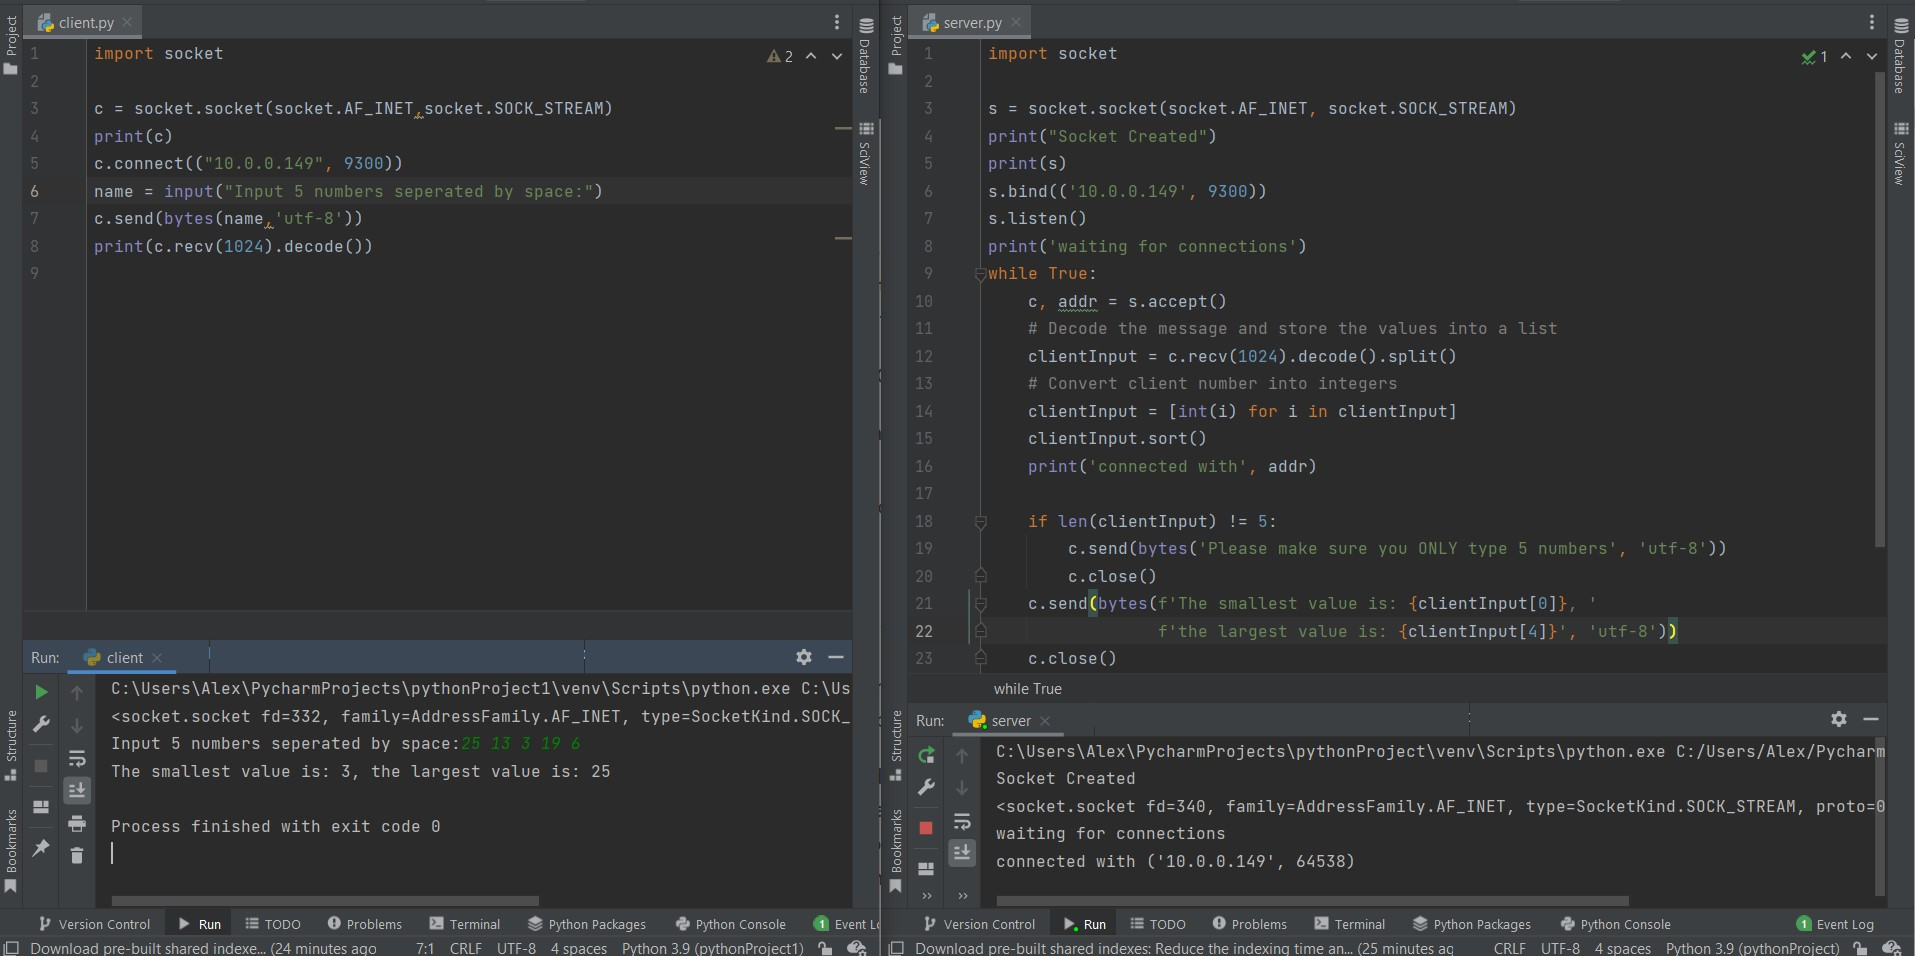
\includegraphics[width=1\textwidth]{q6.jpg}
\end{center}

{\bf Client}
\begin{lstlisting}
import socket

c = socket.socket(socket.AF_INET,socket.SOCK_STREAM)
print(c)
c.connect(('', 9300))
name = input("Input 5 numbers separated by space:")
c.send(bytes(name,'utf-8'))
print(c.recv(1024).decode())
\end{lstlisting}

{\bf Server}
\begin{lstlisting}
import socket

s = socket.socket(socket.AF_INET, socket.SOCK_STREAM)
print("Socket Created")
print(s)
s.bind(('', 9300))
s.listen()
print('waiting for connections')
while True:
    c, addr = s.accept()
    # Decode the message and store the values into a list
    clientInput = c.recv(1024).decode().split()
    # Convert client number into integers
    clientInput = [int(i) for i in clientInput]
    clientInput.sort()
    print('connected with', addr)

    if len(clientInput) != 5:
        c.send(bytes('Please make sure you ONLY type 5 numbers', 'utf-8'))
        c.close()
    c.send(bytes(f'The smallest value is: {clientInput[0]}, '
                 f'the largest value is: {clientInput[4]}', 'utf-8'))
    c.close()

\end{lstlisting}

\bigskip
{\bf Question 7}\\
{\bf (a)}\\
The sequence number of the first segment is the initial value of the sender$\rightarrow$receiver, which is 454.\\
The sequence number of the second segment is $454+105=559$.\\
The sequence number of the third segment is $559+105=664$.\\
The sequence number of the fourth segment is $664+105=769$.\\
The sequence number of the fifth segment is $769+105=874$.

\bigskip
{\bf (a)}\\
The ACK numbers is the sequence number of the next expected segment:\\
Response 1 ACK: 559\\
Since the 2nd segment was lost, the ACK is never sent: x\\
Since the 3rd segment was lost, the ACK is never sent: x\\
Since the 4th segment was lost, the ACK is never sent: x\\
Response 5 ACK: 559\\

\bigskip
{\bf Question 8}\\
{\bf (a)}\\
We can determine the estimatedRTT with $(1-\alpha) \times estimatedRTT + (\alpha \times sampleRTT)$\\
The RTT Deviation can be found with $(1-\beta) \times DevRTT + \beta \times |estimatedRTT - sampleRTT|$\\

\smallskip
First estimatedRTT $=(1-0.125) \times 340msec + (0.125 \times 390msec)=346.25$\\
First RTT Deviation $(1-0.25) \times 29msec + 0.25 \times |340msec - 390msec|=34.25$

\smallskip
Second estimatedRTT $=(1-0.125) \times 346.25msec + (0.125 \times 200msec)=327.97$\\
Second RTT Deviation $(1-0.25) \times 34.25msec + 0.25 \times |346.25msec - 200msec|=62.25$

\smallskip
Third estimatedRTT $=(1-0.125) \times 327.97msec + (0.125 \times 200msec)=311.97$\\
Third RTT Deviation $(1-0.25) \times 62.25msec + 0.25 \times |327.97msec - 200msec|=78.68$\\

\smallskip
{\bf (b)}\\
We can determine the TCP timeout with $estimatedRTT+(4 \times DevRTT)$\\
First TCP timeout $=346.25+(4 \times 34.25)=483.25$\\
Second TCP timeout $=327.97+(4 \times 62.25)=576.97$\\
Third TCP timeout $=311.97+(4 \times 78.68)=626.69$\\

\bigskip
{\bf Question 9}\\
{\bf (a)}\\
GBN:\\
Segments 1, 2, 3, 4, 5 are sent and after the 2nd segment is lost,
segments 2, 3, 4, and 5 are re-sent. So A sends $5+4=9$ segments in total.\\
There  are  4  ACKS  with  sequence  number  1,  and  4  ACKS  with 
sequence numbers 2, 3, 4, and 5. So B sends $4+4=8$ ACKs.\\

SR:\\
A sent 5 segments 1, 2, 3, 4, 5 and then later resent the 2nd segment. So A sends $5+1=6$ segments in total.\\
There are 4 ACKs with sequence number 1, 3, 4, 5, and 1 ACK with sequence number 2. So B sends $4+1=5$ ACKs.\\

TCP:\\
A sent 5 segments 1, 2, 3, 4, 5 and then later resent the 2nd segment. So A sends $5+1=6$ segments in total.\\
There are 4 ACKs with sequence number 2, and 1 ACK with sequence number 6. So B sends $4+1=5$ ACKS.\\

{\bf (b)}\\
If the timeout values for all three protocols are much longer than 5 RTT, then the TCP protocol  will successfully deliver all five data segments in the shortest time interval. This is because TCP uses fast re-transmit without waiting time.\\

{\bf Question 10}\\
{\bf (a)}\\
TCP slow start:\\
During the 1st to 4th transmission round, the congestion windows gradually starts increasing in speed. In the 5th and 6th round, the congestion window exponentially increases during the slow start, thus the operating interval of slow start is from rounds [1,6]. Likewise, from the 23rd to 26th round the congestion window gradually increases, thus the interval of time is from rounds [23, 26].\\

TCP congestion avoidance:\\
From rounds 7 to 16 the congestion window size increases linearly, thus the congestion avoidance interval is [7,16]. Likewise, from the rounds 17 to 22 the congestion window size increases linearly, thus the congestion avoidance interval is [17,22].

\bigskip
{\bf (b)}\\
We can determine segment loss based on the congestion window size after the packet loss:\\
\begin{itemize}
    \item Segment loss is by timeout if the congestion window size is dropped to 1 after the segment loss.
    \item Segment loss is by triple duplicate ACK if the congestion window size is reduced but not dropped to 1 after the segment loss.
\end{itemize}
Since after the 16th transmission round the congestion window is reduced but not dropped to a congestion window size, the segment loss is detected by a triple duplicate ACK.

\bigskip
{\bf (c)}\\
As mentioned in (b), since the congestion window size is dropped to 1 for the segment loss after round the 22nd transmission round, the segment loss is detected by a timeout.

\bigskip
{\bf (d)}\\
The initial value of ssthresh is the congestion window size at the point from which the slow start stops and the congestion avoidance begins. At transmission round 6, the slow start ends, and the congestion avoidance begins. Thus the initial value of ssthresh at the first transmission round is 32.

\bigskip
{\bf (e)}\\
The initial value of ssthresh is the congestion window size at the point from which the slow start stops and the congestion avoidance begins. The ssrthresh value is set to half of its current value in the next tranmission rounds, if segment loss is detected. Segment loss occured at the 16th transmission round. Thus, the ssthresh value is set to half of its size before segment loss. The ssthresh value before segment loss is 42. Therefore, the threshold value is set to half of its size which is 21.

\bigskip
{\bf (f)}\\
Segment loss occurs at the 22nd transmission round, which is before the 24th round. Thus, the ssthresh value is set to half of its size before segment loss. The ssthresh value before segment loss is 29. Therefore, the ssthresh value is set to half of its size which is 14.

\bigskip
{\bf (g)}\\
During the 1st transmission round, packet 1 is sent.\\ 
In the 2nd transmission round, packet 2-3 is sent.\\
In the 3rd transmission round, packet 4-7 is sent.\\
In the 4th transmission round, packet 8-15 is sent.\\
In the 5th transmission round, packet 16-31 is sent.\\
In the 6th transmission round, packet 32-63 is sent.\\
In the 7th transmission round, packet 64-96 is sent.\\
The 70th segment is transmitted during the 7th transmission round.

\bigskip
{\bf (h)}\\
The threshold will be set to half the current value of the congestion window when the packet loss occurs. The value of the threshold and congestion window size when the packet lost occurs is 8. The congestion window will be set to the $new \; threshold \; value + 3MSS$. Thus the new ssthresh value is 4 and the congestion window size is 7.

\bigskip
{\bf (i)}\\
The triple duplicated ACK is received at transmission round 16 which indicates the packet loss. So the packet loss is detected at the 16th round. TCP Tahoe is used for recovery, the congestion window size is set to $1 \; MSS$ after a packet loss.The packet loss occurred at the 16th transmission round, the congestion window size will be set to 1 for the next rounds and the sstrhesh size will be 21 at the 19th round.

\bigskip
{\bf (j)}\\
During transmission round 17, packet 1 is sent.\\
At transmission round 18, packet 2 is sent.\\
At transmission round 19, packet 4 is sent.\\
At transmission round 20, packet 8 is sent.\\
At transmission round 21, packet 16 is sent.\\
At transmission round 22, packet 32 is sent.\\
Total number of packets sent out from 17th to 22nd round is $1+2+4+8+16+32=63$


\end{document}
